% From nature
% The statistical analysis of the data relies on a likelihood formalism, where the likelihood functions describing each of the input measurements are multiplied to obtain a combined likelihood. The observed yield in each category of reconstructed events follows a Poisson distribution whose parameter is the sum of the predicted signal and background contributions. The predicted signal yield is split into the different production and decay processes, so it can be parameterized as a function of dedicated parameters of interest depending on the tested model.

% This chapter presents cross-section measurements of \HWWdet decays, with the Higgs boson produced via the ggF and VBF production mode, using the full dataset collected at \RunTwo of the LHC. 
% Prior measurements of these processes were performed by the ATLAS collaboration. 
% Using data from \RunOne of the LHC the \HWW process was established by reporting its observation with a discovery significance of 6.1 standard deviations~\cite{HIGG-2013-13}. 
% An analysis using a partial \RunTwo dataset reported ggF and VBF production cross sections times \HWW branching fractions of $11.4^{2.2}_{-2.1}$ pb and $0.50^{0.29}_{-0.28}$~\cite{HIGG-2016-07}.
% The analysis presented here uses the full \RunTwo dataset and in addition to the increase in dataset size implements several improvements compared to the previous \RunTwo results. Most noteworthy, the discrimination of the VBF signal is performed using a deep neural network (DNN) instead of a boosted decision tree, ggF events with two or more jets in the final state are included in the measurement, and measurements of cross sections in the kinematic regions defined in the STXS framework are reported for the first time using \HWW events~\cite{HWWPaper}. 
% The analysis is published in \ccite{HWWPaper} and yields some of the most precise Higgs cross-section meausurements to date.\footnote{Comparable results based on the full \RunTwo dataset have also been reported by the CMS collaboration~\cite{Sirunyan_2021}.}
% The results are also used as input to a combined Higgs boson measurement published in \ccite{NaturePaper} where they make an essential contribution.

% This is obseved:
% $11.4^{2.2}_{-2.1}$ pb and $0.50^{0.29}_{-0.28}$
% 12.0 ± 1.4 pb and 0.75 +0.19 −0.16 pb,

The full \RunTwo dataset of the LHC recorded by the ATLAS experiment corresponds to 139\,\ifb\ and allows for precise measurements of ggF and VBF Higgs boson production cross-sections at $\sqrt{s} = 13\,$TeV.
All measurements presented are consistent with the SM predictions. 
% The measurement of in total 11 Higgs boson production cross sections split in different kinematic regions have been performed by the ATLAS collaboration for the first time using \HWW decays. 
The measurement of in total 11 STXS cross sections have been performed by the ATLAS collaboration for the first time using \HWW decays. 
While the results of the inclusive cross-section measurements are largely dominated by systematic uncertainties, the measurement of 6 of the 11 STXS cross sections are still dominated by statistical uncertainties. 
Furthermore, the VBF production mode is observed with a discovery significance of above $5\,\sigma$\footnote{A significance of at least $5\,\sigma$ above the background expectation is commonly considered an observation in particle physics.} for the first time using only \HWW decays.

% Previous \RunTwo results of the ATLAS collaboration reported corresponding cross sections of the ggF and VBF production mode of $11.4^{2.2}_{-2.1}$~pb and $0.50^{0.29}_{-0.28}$~pb~\cite{HIGG-2016-07}.
\subsection{Comparison to previous results}
Previous \RunTwo measurements of the ATLAS collaboration that used a dataset corresponding to 36\,\ifb\ reported cross sections of the ggF and VBF production mode of $11.4^{+2.2}_{-2.1}$~pb and $0.50^{+0.29}_{-0.28}$~pb\footnote{Broken down into statistical and systematic uncertainties the results are $\sigmaGGF = 11.4^{+1.2}_{-1.1}\,\text{(stat.)}^{+1.8}_{-1.7}\,\text{(syst.)}$~pb and $\sigmaVBF= 0.50^{+0.24}_{-0.22}\,\text{(stat.)}\pm 0.17\,\text{(syst.)}$~pb, respectively}, respectively~\cite{HIGG-2016-07}.
The measurements presented here thus result in a 40\% and 60\% smaller total relative uncertainty on the ggF and VBF measurement, respectively. In part, this improvement is due to the increased size of the dataset by almost a factor of four.
In addition, the ggF measurement benefits from the inclusion of the ggF \TwoJet category and the VBF measurement is drastically improved by the implementation of a DNN as final fit discriminant. 

The previous analysis, which used a boosted decision tree (BDT) for the VBF signal discrimination, reached an expected discovery significance of $2.6\,\sigma$ for the VBF signal, which is to be compared to $6.2\,\sigma$ achieved by the analysis presented. 
Direct comparisons between the performance of the BDT and the DNN with an otherwise identical analysis strategy showed an improvement of about 20-30\% in the discovery significance depending on the binning choice of the fit discriminant. % solely due to the change of the discriminant. 
%These developments allowed observing the VBF production mode of the Higgs boson for the first time using only \HWW decays.

Both the ggF and VBF measurements also benefit from improvements in the estimation of the background from misidentified leptons, substantially reducing their impact on the measurement with respect to the previous results. 
Furthermore, improvements in ATLAS reconstruction software, identification algorithms, and improved object calibration measurements are of benefit. 
An example of the latter is the JER measurement presented in \cref{chap:calibration}. 

\subsection{Impact of analysis in combined measurements}
The analysis presented is also crucial input to combined Higgs boson measurements~\cite{NaturePaper}, which incorporate various analyses other than the one presented that study different combinations of Higgs boson production and decay processes. These results are summarized in \cref{chap:higgs}.
% The ones with the largest contributions are analyses of $H \to ZZ$, $H \to \gamma\gamma$, and $H \to \tau\tau$ decays that consider Higgs boson production via all major production modes. 
The combined measurements of both inclusive VBF and ggF cross sections as well as STXS cross sections benefit greatly from the inputs of the \HWW analysis.
In particular, measurements of \HWW decays provide the most precise measurements of the coupling of the Higgs boson to vector bosons, especially due to the VBF measurement, since the $HVV$ vertex appears twice in the VBF, \HWW diagram (see \cref{sec:signal-bkg-characteristics}). 
Using the $\kappa$-framework, the $HV$ coupling-strength modifier is measured to be $\kappa_{V} = 1.035 \pm 0.031$, assuming the same modifier for the $HW$ and $HZ$ coupling.
Treating the $HW$ and $HZ$ coupling independently, the $HW$ coupling is measured with relative uncertainties of about 5-10\%, depending on the model assumed. 
All results of the combined measurements are found to be consistent with the SM expectations, thereby setting strong constraints on couplings to new particles beyond the SM.  
% The predicted signal yield is split into the different production and decay processes, so it can be parameterized as a function of dedicated parameters of interest depending on the tested model.

\subsection{Future improvements}
Due to the increased size of the available dataset, uncertainties from theoretical sources have become the bottleneck for many of the \HWW measurements presented.
In particular, the VBF measurement is largely dominated by signal theory uncertainties, mainly due to the parton shower modelling.
A better understanding of parton shower effects and more accurate theoretical calculations are therefore crucial to improve the measurements in future iterations.~\cite{Jger2020} 

A larger dataset collected in future Runs of the LHC is still expected to improve the measurements, in particular the STXS measurements targeting EW $qqH$ production, the majority of which are still largely limited by statistical uncertainties. 
More data will also help to both improve the estimation of theory uncertainties and to better control the extraction of the normalization of backgrounds from CRs. 

Changes to the analysis strategy may also improve the measurements. 
Currently, the ggF SRs are defined with simple analysis selections. Instead, using a DNN-based approach to separate the ggF signal from the backgrounds could prove beneficial. 
A larger signal-to-background ratio in the ggF-sensitive regions will also reduce the impact of systematic uncertainties. 
Furthermore, the current ggF and VBF \TwoJet SRs use very similar kinematic and topological selections but are made orthogonal by requirement on the CJV and OLV (see \cref{sec:event-categorization}). The latter selection is found inefficient in particular for the ggF \TwoJet category, where about 30\% of ggF signal events are removed from the ggF SR due to this requirement. 

For the above-mentioned reason, the author of this thesis studied using a modified analysis strategy for the \TwoJet categories, aiming at both a better separation of ggF signal events from the backgrounds and an improved separation between the ggF- and VBF-sensitive regions. 
Both goals can be achieved by using a multiclass classifier that distinguishes between ggF signal events, VBF signal events, and background events. 
To this end, a DNN is trained with three output nodes that separately target the ggF signal (\emph{DNN ggF output}), VBF signal (\emph{DNN ggF output}), and the backgrounds. 
A two-dimensional discriminant can then be defined based on the DNN ggF output and DNN VBF output.
This discriminant is shown in \cref{fig:2d-discriminant} for the expected ggF yields, VBF yields, and background yields, and shows a good separation of the signals while discriminating the backgrounds. 
The discriminant is shown in a newly defined common \TwoJet SR that is tested for use in the measurement of both the ggF and VBF signal. 
The details of the selections are provided in \cref{app:multi-class-2jet-strategy}. 
The performance of this new approach is investigated by comparing the results of the 2-PoI fit to the Asimov dataset, only using the \TwoJet categories as inputs. 
The ggF and VBF signal strengths are found to have smaller uncertainties by 20\% and 7\%, respectively, when the proposed new definition of the \TwoJet categories is used. 
The improvements for the ggF measurement are mostly due to the change of the discriminant to a DNN, but also benefit from the more efficient separation between the ggF- and VBF-sensitive regions. 
The small improvements in the VBF measurement are due to a slightly finer binning in the VBF-sensitive region. 
While these studies should be considered preliminary and need further scrutiny, this redefinition of the \TwoJet categories seems a promising way forward for future analyses of \HWW decays.

\captionsetup[subfloat]{captionskip=5pt} % space between subfloat caption and image
\begin{figure}[ht]
    \centering
    \subfloat[]{
        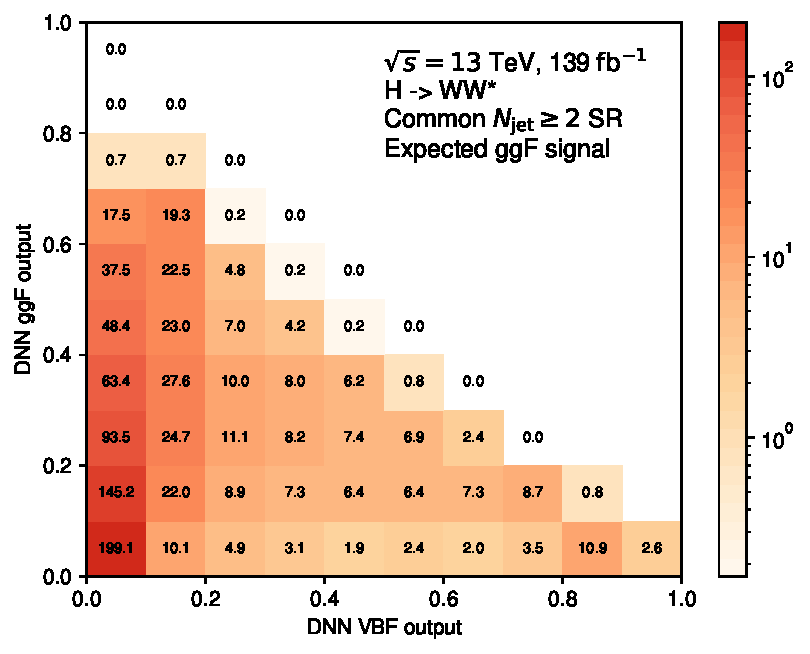
\includegraphics[width=0.48\textwidth]{figures/hww/2d-discriminant/ggF_signal_Heatmap_VBF_vs_ggF.pdf} \hfill
    } 
    \subfloat[]{
        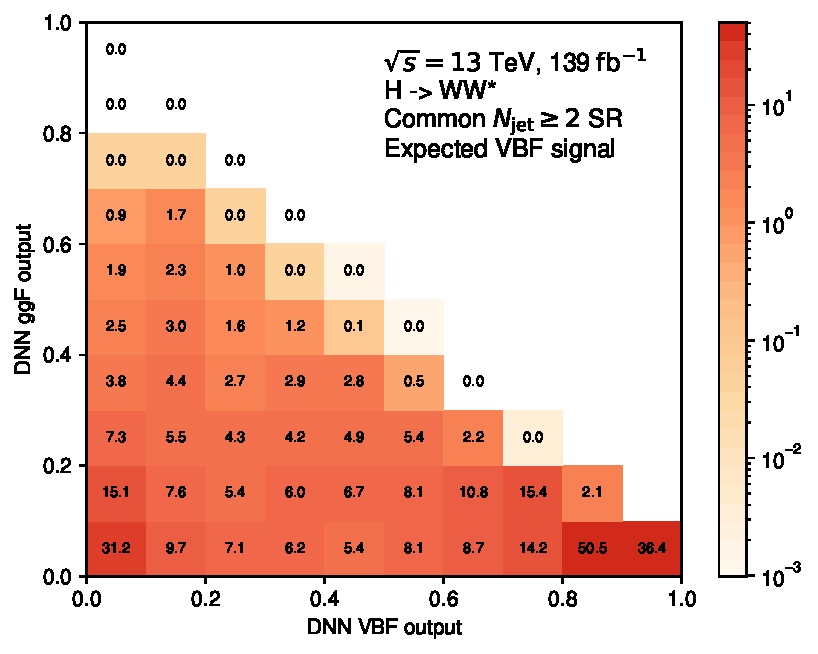
\includegraphics[width=0.48\textwidth]{figures/hww/2d-discriminant/VBF_signal_Heatmap_VBF_vs_ggF.pdf} \hfill
    } \\
    \subfloat[]{
        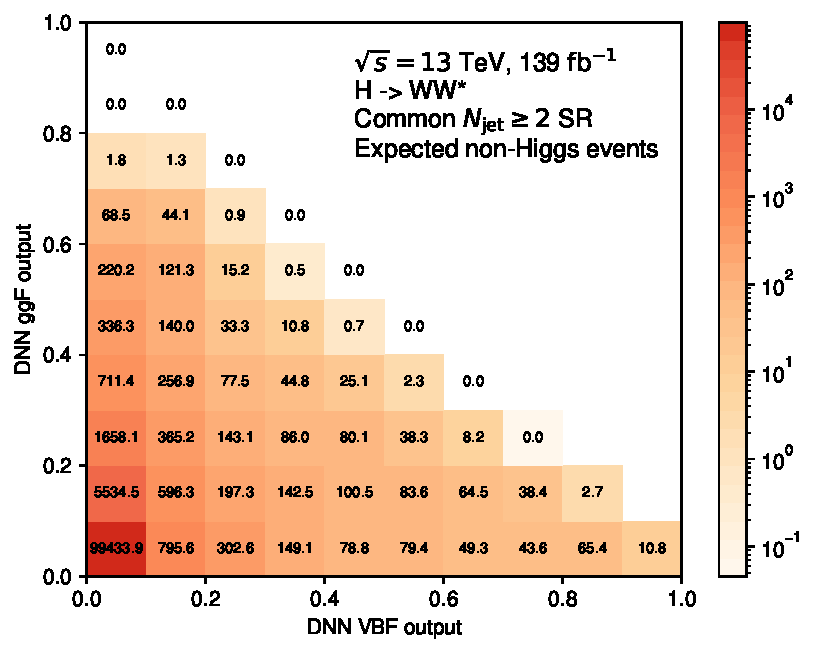
\includegraphics[width=0.48\textwidth]{figures/hww/2d-discriminant/non-Higgs_events_Heatmap_VBF_vs_ggF.pdf} \hfill
    }
    {\caption{Two-dimensional distribution of the DNN ggF output vs the DNN VBF output for the (a) ggF signal, (b) VBF signal, and (c) total background from non-Higgs boson events, shown in a common \TwoJet category for the ggF \TwoJet and VBF analysis. 
    \label{fig:2d-discriminant} }}
\end{figure}